%4. Problem space (Prototype, test setups, existing software)
\chapter{Understanding the Problem Space}
\label{chap:understanding-the-problem-space}
In order to provide a satisfying solution to the problem at hand, the problem itself and the environment it occurs in must be researched. This chapter aims to explore and examine the problem space, resulting in a set of artefacts (namely a domain model and a set of requirements) that aid in understanding the context and designing an appropriate solution. First, a prototypical network proxy is designed and implemented in section \ref{sec:prototypical-implementation} to get an understanding of the problems and challenges involved in designing, implementing and using such software. Based on these experiences, interviews with experts in penetration testing are conducted and evaluated in section \ref{sec:interviews} to get a proper understanding of their everyday work and resulting problems. Lastly, existing software that aims to intercept communication for various scenarios and technologies is examined in section \ref{sec:analysis-existing-software}, compared to each other and their usefulness for the problem-specific scenarios is assessed.

\section{Prototypical Implementation}
\label{sec:prototypical-implementation}
The prototype was designed to be used in two realistic scenarios; one in an \ac{ICS} context and a more complex one in a cloud context. The goal of this section was to implement a prototype that could be used to intercept communication between an \ac{IoT} device and its cloud service as shown in figure \ref{fig:network-communication-diagrams}. It was developed incrementally so individual components could be derived from requirements, designed, implemented and evaluated in fixed sprints.

\begin{figure}%
    \centering
    \subfloat[\centering Regular communication between an \ac{IoT} device and a cloud service.]{{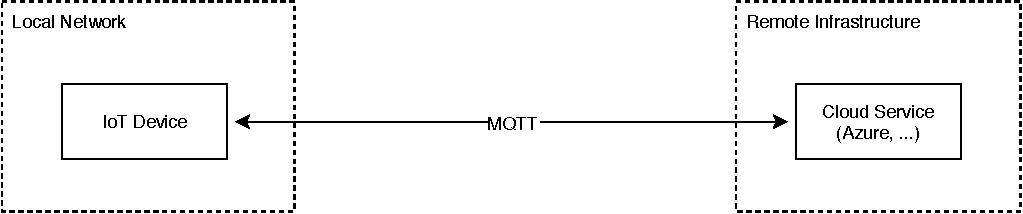
\includegraphics[width=10cm]{img/ch04/Setup - 1 Regular.pdf} }}%
    \qquad
    \subfloat[\centering Communication intercepted by a \ac{MITM} proxy.]{{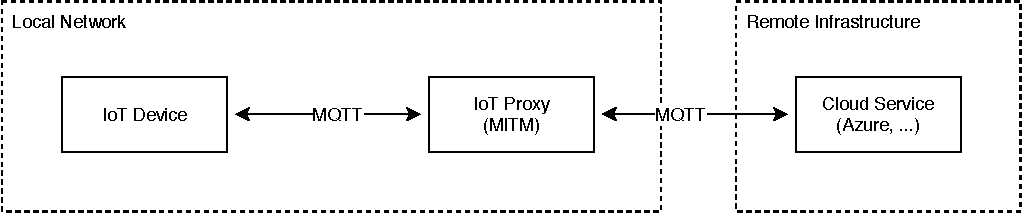
\includegraphics[width=10cm]{img/ch04/Setup - 2 Pentesting.pdf} }}%
    \caption{Installing a \ac{MITM} proxy to intercept network communication for penetration testing.}%
    \label{fig:network-communication-diagrams}%
\end{figure}

\subsection{Example Scenarios}
The following scenarios describe realistic configurations of \ac{IoT}/\ac{IIoT} devices that should be tested with the prototype:

\paragraph{Scenario \#1: \ac{ICS} Modbus \ac{TCP}}
In this \ac{IIoT} scenario, a \ac{HMI} (\emph{Siemens KTP400 Basic}) sends commands to and receives data from a \ac{PLC} (\emph{Siemens S7-1200}) using Modbus \ac{TCP}. The \ac{PLC} continually counts up a value up to 100 and begins anew at zero while the \ac{HMI} displays the current value and provides a button that, upon being pressed by a user, resets the current value to zero. \\
In this scenario, attackers could perform a variety of attacks on the system by intercepting and manipulating network traffic, for example:
\begin{itemize}
    \item By dropping messages sent from the \ac{PLC} to the \ac{HMI}, the application may appear unresponsive as new data is not displayed on the \ac{HMI}. In production environments, this could lead to dangerous situations as sensor readings that indicate harmful environmental conditions would not be presented to supervising personnel. 
    \item When dropping messages sent from the \ac{HMI} to the \ac{PLC}, control commands can be suppressed. This attack can result in catastrophic situations when emergency shutdowns issued by supervising personnel is not registered by the affected machines.
\end{itemize}

Due to the rather simple nature of the Modbus \ac{TCP} protocol, intercepting and manipulating communication is expected to be trivial. %TODO: Add diagram?
%https://support.industry.siemens.com/tf//WW/en/posts/s7-1500-communication-and-modbus-tcp-on-hmi/144092?page=0&pageSize=10
%https://support.industry.siemens.com/cs/pd/379924?pdti=td&dl=en&lc=en-DK

\paragraph{Scenario \#2: \ac{AWS} \ac{IoT}} This \ac{IoT} cloud scenario utilizes a local \ac{IoT} device that is integrated into the \ac{AWS} \ac{IoT} platform. The device connects to the cloud platform, authorizes itself via \ac{HTTP} and upgrades the \ac{HTTP}-connection to a \ac{WS} stream upon successful authorization. It eventually communicates to a remote \ac{MQTT} broker by tunnelling \ac{HTTP} over the \ac{WS} stream. At this stage, it can publish information such as sensor readings to \ac{MQTT} topics or subscribe topics and react on incoming value changes. \\
%Specific scenario? Which device is used? Which use cases does it serve?
%TODO: Add possible attacks
This scenario makes use of three communication protocols, uses these protocols dependent on the state of authentication (as seen in \ref{fig:aws-statemachine}) and even tunnels one protocol through another one. Therefore, testing communication in this scenario is expected to involve more complex approaches than the first one. %TODO: Add diagram?

% State machine
\begin{figure}[ht] 
    \centering
    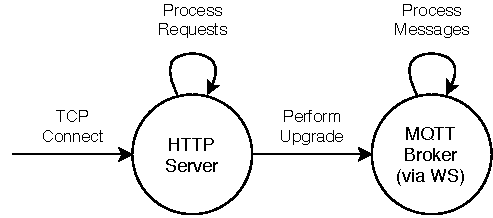
\includegraphics[width=6cm]{img/ch04/Statemachine 2.pdf}
    \captionof{figure}{State machine of \ac{AWS} \ac{IoT} communication}
    \label{fig:aws-statemachine}
\end{figure}
% Reference: https://aws.amazon.com/blogs/aws/aws-iot-cloud-services-for-connected-devices/


\subsection{Requirements}
To be able to operate in both of the aforementioned scenarios, the prototype had to implement a set of functional requirements:
\begin{itemize}
    \item [\textbf{F1}] \textbf{Protocols:} The software must implement parsing/crafting messages/packets of the following communication protocols: \ac{HTTP}, \ac{WS}, \ac{MQTT} and Modbus \ac{TCP}. \\
    \textit{Fit criterion: TBD} %TODO: Write fit-criterion
    \item [\textbf{F2}] \textbf{Network Stacks:} The software must be able to parse protocols that are tunnelled through other protocols (\enquote{\emph{stacked}}). It must provide an interface to the user where they can specify which communication protocols are used and whether and how they are stacked (further referred to as \emph{network stack}).\\
    \textit{Fit criterion: The software processes a configuration file that lets users specify which protocols to be used and whether/how they are stacked.} 
    \item [\textbf{F3}] \textbf{State Machine:} The software must be able to switch network stacks dependent on configurable \emph{states}. It must provide an interface for the user to specify when to switch to using another network stack, represented using state machines and rule sets for transmission between states.\\
    \textit{Fit criterion: The software processes a configuration file that lets users specify when to switch between network stacks.}
    \item [\textbf{F4}] \textbf{Integration:} The software shall provide interfaces for integration of third-party software.\\
    \textit{Fit criterion: The software allows sending requests/responses to \enquote{Burp Suite} for manipulation.}
    \item [\textbf{F5}] \textbf{Scripting:} The software shall provide scripting capabilities for automated manipulation of messages/packets.\\
    \textit{Fit criterion: Users can define script-snippets to be executed on messages/packets.}
\end{itemize}

The following non-functional requirements were defined:

\begin{itemize}
    \item [\textbf{N1}] \textbf{Extensibility:} To allow for future implementation of further communication protocols the software shall be implemented in a modular fashion.
    \item [\textbf{N2}] \textbf{Platform Compatibility:} In order to support a broad spectrum of target platforms, the software shall be implemented platform-independently.
    \item [\textbf{N3}] \textbf{Reusability:} The software shall be reusable so it can be used in future tests that may feature new configurations of network stacks.
    \item [\textbf{N4}] \textbf{Open Source:} The software shall be available as open source software so programmers and members of the IT community may contribute to improving it.  
\end{itemize}

Due to this implementation serving as a prototype and being of an academic nature, no specific constraints were defined. It was to be developed strictly ignoring aspects of usability and stability as it should not be used in production environments but in laboratories exclusively.

\subsection{Design}
The prototype was designed to be fit for use in the second scenario as, regarding network communication, it was more complex than the first one. Specifically, the second scenario demanded the implementation of the network stack and a state machine to switch between states and process protocols dependent on thereon.\\
Parsing protocols that were tunnelled through other protocols appeared to be a potentially challenging requirement. In order to tackle it, a variation of the /\emph{\enquote{pipeline}} (sometimes referred to \emph{\enquote{pipes and filters}}) design pattern was used as can be seen in \ref{fig:design-pipes-and-filters}. It was designed to be used as follows:
\begin{enumerate}
    %\item Messages originate from an initial pipe (e.g. raw bytes are received from a \ac{TCP} socket).
    %\item Pipes forward messages to an attached \emph{filter} that performs operations on the messages such as parsing protocol packets from the messages' data
    %\item If the current pipe has a succeeding pipe, the modified/parsed messages are sent to it, thus initiating another modification/parsing step. If however the current pipe lacks a succeeding pipe, the modified/parsed messages' direction is reversed and sent back to the previous pipe.
    %\item Pipes send messages through their attached filter to effectively serialize the messages' data back to the protocol that was initially received at the first pipe.
    \item Data sent to a \emph{pipe} is processed by its associated \emph{filter}. 
    \item Filters can manipulate the data, for example parsing protocol-specific packets from raw binary data or serializing packets back to binary data.
    \item After processing, pipes route data either to the succeeding pipe or, in case a pipe does not have a succeeding pipe associated to it, back to its previous pipe.
    \item Eventually, data is deserialized and manipulated on multiple levels and serialized back to the originating format.
\end{enumerate} %\emph{pipes} would forward data to \emph{filters}.

% TODO: Explain Figure A1 \ref{fig:app-diag-pipesfilters-1} and A2 \ref{fig:app-diag-pipesfilters-2}.

% State machine (States, Transitions, Rules)
% Network Stack (Stack, Pipes, Filters, Encoders)
% Messages (MessageDirection, Payload, PayloadTypes)
% 
\begin{figure}
    \centering
    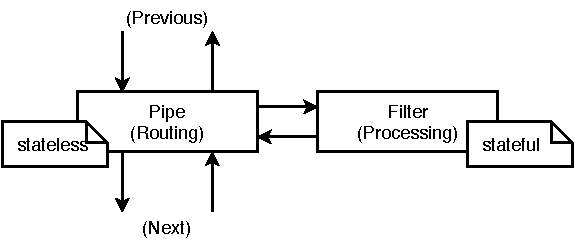
\includegraphics[width=6cm]{img/ch04/Architecture - Pipes and Filters.pdf}
    \captionof{figure}{The variation of the \emph{\enquote{pipes and filters}}/\emph{\enquote{pipeline}} design pattern used in the prototype.}
    \label{fig:design-pipes-and-filters}
\end{figure}

% TODO: References Pipes & Filters \ref{fig:app-diag-pipesfilters-1} \ref{fig:app-diag-pipesfilters-2}




\subsection{Implementation}

\subsection{Insights Gained}
\begin{itemize}
    \item Due to the \ac{MTU}, large messages are broken into chunks that are transferred sequentially. This requires the proxy to work on streams of incoming data and reassemble messages from said chunks.
    \item Support of multiple clients is non-trivial as communication between clients and servers is not necessarily connection-oriented (e.g. \ac{HTTP}). Question: Do penetration testers need to test multiple devices at the same time?
    \item Increasing the size of the payload of a messages can result in the payload being split upon multiple messages (e.g. \ac{WS}). Question: Do penetration testers require exact control over the implementation of protocols?
    \item Manipulating messages, on the fly via scripting or by hand using third-party integrations (e.g. to \emph{Burp Suite}), can introduce latency to the communication. Question: Are there strict timing requirements during penetration tests?
    \item Many libraries offer high-level functions to the programmer while avoiding exposure of low-level functionalities like crafting or parsing messages.
\end{itemize}

%\begin{figure}[t]
%    \centering
%    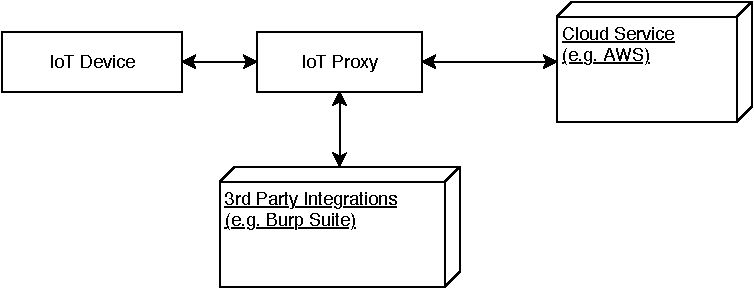
\includegraphics[width=6cm]{img/ch04/Architecture - Simple.pdf}
%    \captionof{figure}{High-level Software Architecture}
%    \label{fig:high-level-software-architecture}
%\end{figure}

%\begin{figure}[t]
%    \centering
%    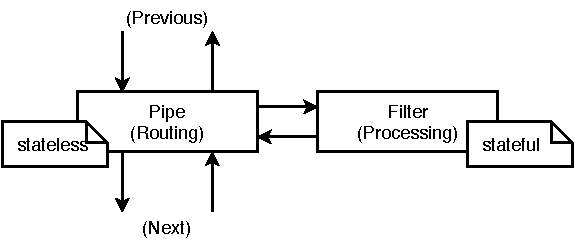
\includegraphics[width=6cm]{img/ch04/Architecture - Pipes and Filters.pdf}
%    \captionof{figure}{"Pipes and Filters" Design Pattern}
%    \label{fig:design-pattern-pipes-and-filters}
%\end{figure}



\emph{TBD; implementation is completed, needs to be written down; include its diagrams} %TODO Write down implementation 

\section{Interviewing Experts for Insights}
\label{sec:interviews}
Interviews may be an efficient way to get an expert’s opinion on something they are a professional in. Thus, expert interviews were conducted to let security researchers give insight into their everyday work and the challenges they face. The information and insights gathered in these interviews were then used to model a persona, various work scenarios and use-cases that as a whole aim to represent their work.

\subsection{Interview Guideline}
An interview guideline (shown in \emph{TBD}) %TODO: Reference appended interviews
was created to keep focus on key points during interviews so that interviewees would not stray too far from the relevant points. The guideline also served as a checklist so the interviewer could make sure that all questions and points that should be covered  initially, were in fact covered by the end of the interviews. It was composed of three sections:

\paragraph{1. Experiences with IoT} The answers to these questions would give insights into what kind of applications the security researchers had worked on in the past. Answers to question \emph{1.1.} were of particular interest as they might represent what technologies were being examined by security researchers and may be popular in today’s applications.
\paragraph{2. Processes in Everyday Life} This section aimed to cover questions about the processes and tasks security researchers perform during penetration tests of IoT applications in their everyday life. Ideally, answers to those questions would show the approaches taken and challenges faced during their work, uncovering potential needs and underlying motivation.
\paragraph{3. The Future of IoT} This section had security researchers assess what the future of IoT may be like from their point of view. This required the interviewees to make a critical assessment of the status quo.

%The experience gained from implementing the prototype in \ref{sec:prototypical-implementation} greatly influenced the creation of this guideline. For example question \emph{1.3. Were there any special constrains (e.g. real-time systems) when working with them?} 

%Some of the questions in these sections originated from or were influenced by experience gained when implementing the prototype proxy application in \ref{sec:prototypical-implementation}. 

\subsection{Conducting Interviews}
Interviews were conducted with six %Patrick, Cédric, Théo, Oliver, Pierre, Jonah
\emph{NVISO} employees that all had worked on security assignments on \ac{IoT} or \ac{IIoT} applications in the past. There is considerable variety in
\begin{itemize}
    \item the experience they had in working on security assignments in general: all interviewees had a strong background in cyber security that reached back multiple years except one who was a working student at \emph{NVISO Labs}.
    \item and the experience they had in working on \ac{IoT}/\ac{IIoT} applications: two interviewees worked on assessing \ac{IoT}/\ac{IIoT} applications only occasionally, one was part of a car manufacturer's automotive security team and three were part of \emph{NVISO Labs} and worked with smart devices on a regular basis.
    % Position? CEO vs. Consultant vs. Working student
    % 
\end{itemize}
The duration of the interviews varied from 45 minutes to two hours depending on the amount and level of detail of information provided by the interviewees and the number of times that the interviewer had to ask further questions.

\emph{TBD: Summary of the interviews and conclusions drawn + personas and use cases}

\section{Analysis of Existing Software}
\paragraph{Wireshark} 3,690,000 lines of code\footnote{This number was returned by the \emph{cloc} utility run on commit \emph{3a8111e1c2adcdc0603993c6ed5d20a40f162125} of Wireshark's Github mirror.}\emph{TBD}
\paragraph{MITMf} \emph{TBD}
\paragraph{Ettercap} \emph{TBD}
\paragraph{bettercap} \emph{TBD}
\paragraph{mitmproxy} \emph{TBD}
\paragraph{mProxy} \emph{TBD}
\paragraph{IOXY} \emph{TBD}

\emph{TBD; planned: paragraph about each program including a general description, uses, capabilities and usefulness} %TODO
\label{sec:analysis-existing-software}
\begin{table}[h]
    \centering
    \begin{tabular}{r|c|c|c|c|c|c}
        \toprule
              \thead{$Name$} & \thead{$Latest$\\$Release$} & \thead{$Implemented$\\$in$} & \thead{$Supported$\\$Protocols$} & \thead{$R$} & \thead{$W$} & \thead{$D$}\\
        \midrule
            Wireshark & 2020-07-01 & C & Various & \cellcolor{green!25}Y & \cellcolor{red!25}N & \cellcolor{red!25}N \\
        \midrule
            MITMf & 2015-08-28 & Python & Various & ? & \cellcolor{green!25}Y & \cellcolor{green!25}Y  \\ %https://github.com/byt3bl33d3r/MITMf
        \midrule
            Ettercap & 2019-07-01 & C & Various & \cellcolor{green!25}Y & \cellcolor{green!25}Y & \cellcolor{green!25}Y  \\
        \midrule
            bettercap & 2020-03-13 & Go & Various & \cellcolor{green!25}Y & \cellcolor{green!25}Y  & \cellcolor{green!25}Y \\
        \midrule
            mitmproxy & 2020-03-13 & Python & HTTP/S, WS & \cellcolor{orange!25}P & \cellcolor{orange!25}P & \cellcolor{orange!25}P \\ %https://github.com/mitmproxy/mitmproxy
        \midrule
            mProxy & Pre-Releases only & Go & MQTT & ? & \cellcolor{green!25}Y & - \\ %https://github.com/mainflux/mproxy
        \midrule
            IOXY & Source only & Go & MQTT & \cellcolor{green!25}Y & \cellcolor{green!25}Y & \cellcolor{green!25}Y \\ %https://github.com/mainflux/mproxy
        \bottomrule
    \end{tabular}
    \caption[Comparison of existing software]{Comparison of existing software where $R$, $W$ and $D$ describe read, write and deletion capabilities, respectively. $Y$, $N$ and $P$ indicate full, no or partial functionality, respectively.}
    \label{table:comparison-existing-software}
\end{table}